\documentclass{article}
\usepackage{graphicx}
\usepackage{amsmath}
\usepackage{mathtools}
\usepackage[margin=1in]{geometry}
\setlength{\parindent}{0in}
\author{Graham Roberts}
\title{Research Update}
\begin{document}
\maketitle
\section{introduction}
This week I spent attempting to get everything ready for actual analysis.  I did analyze the parallax data, but that did not prove very fruitful.  There were zero matches to within three arcseconds of any known members, and only siz stars within the tidal radius of the cluster, that also had even remotely reasonable proper motions.  I have not computed a proper membership probability for them, or added them to my known catalog, but that option is on the table if we think those five or so stars are worth the time.  Most of my work has been put into fitting the PARSEC models.  

\section{PARSEC fit}
I have only started with the fitting process.  My first task was downloading the models, which was fast, but they were  bit tricky to work with.  The file was in the form of several tables in one file separated by repeated header information.  This made it impossible to simply read it in with numpy, and I had to actually read it line by line separating bits out with python.  Needless to say I now have all the model resting comfortably in a beatiful database of isochrones searchable by age.  Being that they are at absolute magnitude and we only have apparent magniudes in our observations, I implmented the distance modulus.  Since we were unsure of distance (seeing estimates from 170 to 190 parsecs) I performed my own fit to the models in order to estimate distance.  My current best fit only places the cluster at 145 parsecs, which is confusing me.  I currently have a more in depth loop checking my conclusion, but that could take the night and it will almost certainly support my conclusion.  Here is a model of my known members plotted along with every isochrone in the range of 30 million years to 200 million years.  I've shifted the isochrones to 145 parsecs.  Also when performing my best fit I only fit according to stars along the main sequence, which has the most certainty and wouldn't influence my future selection of models much.

\begin{center}
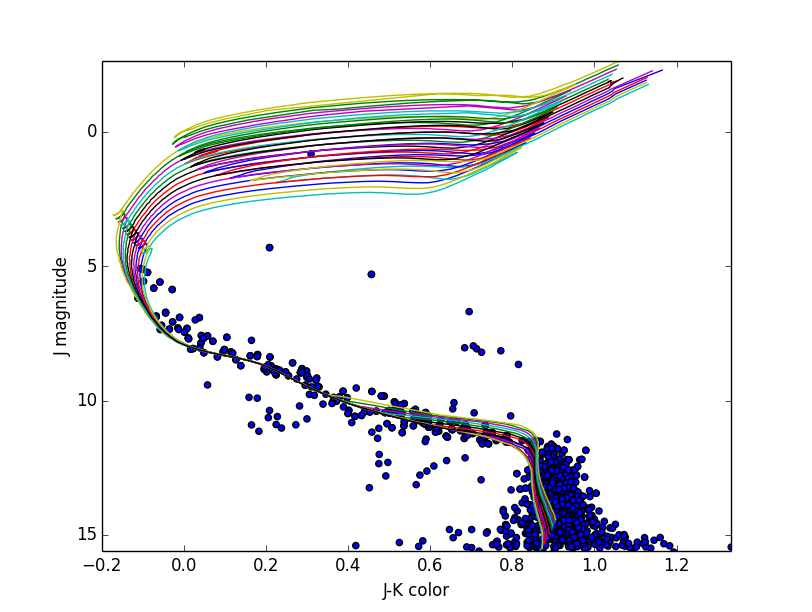
\includegraphics[width=.8\textwidth]{modelfit}
\end{center}

\section{Next Steps}
I still need to fit an isochrone to my data.  This should be faster than the linear shift since I already have most of the functionality written.  Also there are only 14 discreet options to check where as the distance calculation was over a continuous range.  That said once we have found the closest matches I believe it would be prudent to create a continuous model on the small range and match there so as not to be forced into one of the specific ages hat the PARSEC madels are in.  I'm pretty sure that's what you had in mind, but we haven't discussed that in detail yet.  I am also unsure of what distance we should place the models at.  My estimate of 145 parsecs it crude and based off of isochrone shifts, which I place less faith in than the Hipparcos re-reduction.  It does however fit our data a little bit better.  I am also questioning the uncertainty of the models.  particularly in the faint star region.  The models show differences there which is encouraging, but my data is not very amiably to a single sequence.  Considering the difficulties logically asociated with measurement of stars that are either extremelly bright or pretty dim, I would not be surprised if that portion was not particularly ideal for fitting.  There are a couple stars just brighter than the main sequence at the turn off.  These are what we are planning on fitting with, but there's only a handful, so our uncertainty will be high.  Additionally there are some stars in this region, that I believe should fall somewhere on the isochrones, they are however a little too red for that.  There are a number of different reasons that they could be observed as redder than they need to be.  Should we analyze the reddening and possible redshift of he stars.  Over the next couple days I will impliment the Mermillod, and Markarov.  If you can get members from Marcel, that would also come in handy.  I am almost certain I should still force as many of the sars based off of parallax into my catalog as I can.  Lastly I may put some of our candidate members in the fit.  I still cannot find a good place to really make the cut, but I might be able to find a few stars in the correct color-magnitude range that also match membership criteria beyond too much doubt.
\end{document} 
